\documentclass[main.tex]{subfiles}
\begin{document}


\chapter{Concept} \label{chap:Concept}


\begin{figure}[H]
    \centering
    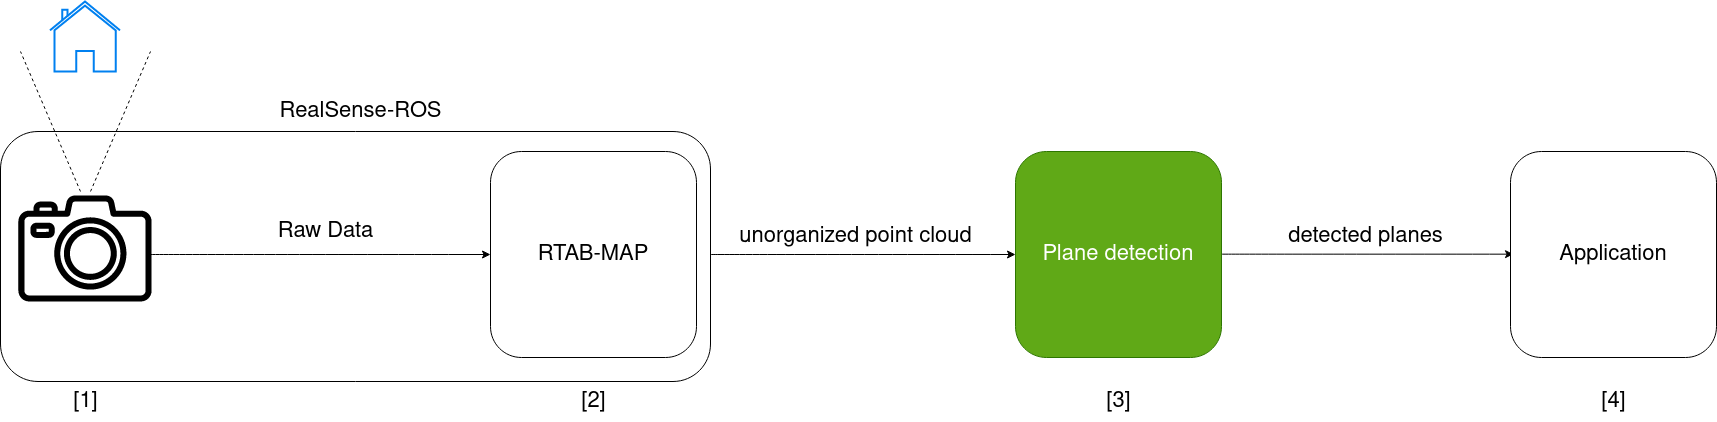
\includegraphics[width=15 cm]{images/concept_specific.png}
    \caption[Concrete Concept Graphic]{The procedure of the plane detection process. The specialized sensor records data ([1]), which is passed to
        a SLAM algorithm ([2]). After map assembly, a point cloud is handed to a plane detection algorithm ([3]).
        The detected planes are given to a use-case-specific application ([4]).}
    \label{fig:concept}
\end{figure}

% FIXME direkt die spezifische nehmen und im folgenden erklären wie ich dazu komme
% FIXME ebenen zurück in die scene / transformation / tracking oder so 
% FIXME formale korrektheit der grafik: 
% \section{Scenario / UseCase}

% Within a given use case or scenario that involves the detection of planes, the user records the surroundings with a camera. The raw data is then either
% directly, or after some preprocessing steps, passed to a plane detection algorithm, which then hands the detected planes to an application for further use.
% This application could use those planes to define the playable area in an augmented reality (AR) video game or alternatively build a digital floor
% plan, or 3D model, of an apartment.

% Especially in scenarios where the user moves through the environment, the time between recording and the planes reaching the application is crucial.
% If an autonomous robot moves through an apartment complex, the delay must be as short as possible to avoid a collision with a wall the robot has not yet detected.
% The problem can therefore be defined in such a way that planes must be detected in real-time and at the same time be sufficiently precise for the given use case.

% % To optimize the entire process, shown in Figure~\ref{fig:concept}, this work will aim to answer the question of to what extent precise real-time plane detection is feasible. 
% % NOTE alternative: 
% To optimize the entire process, shown in \ref{fig:concept}, this work is focused on the plane detection step (green).

% Furthermore, we focus on indoor environments, as motivated by Chapter~\ref{chap:Introduction}.
% This includes the buildings we encounter in our normal lives, whether it is the home we live in, the office we work in, or a stripped-down version of a building during construction.



% Viele Anwendungsfälle bauen auf das finden von ebenen in realen strukturen auf. Es werden spezielle sensoren entwickelt, welche extrem präzise daten der aufgenommenen umgebung liefern können.
% Mit dieser präzision steigt natürlich auch der preis, was sich natürlich nicht jeder leisten kann. Ein Nutzer möchte und kann sich wahrscheinlich nicht einen 4000 Sensor leisten, nur um AR spiele in seinem Wohnzimmer zu spielen.
% Dazu kommt oft eine zeitliche komponente. Wenn sich der nutzer durch die umgebung bewegt möchte dieser nicht 

% FIXME vertiefen: (aus INTRO) "Problem an letzterem: nicht möglich einen einheitlich besten algorithmus auszuwählen"  

Roter Faden:
\begin{itemize}
    \item generic view on AR + VR system
    \item Describe the building blocks in there
    \item Point out that the decision on the "best" PDA is not clear
    \item Tell me why that is not clear!
    \item Get me going on those PDA
          \begin{itemize}
              \item describe my view on the world
              \item show marco that table
              \item describe what these values mean and why they are important
          \end{itemize}
\end{itemize}

\section{Selection of Plane Detection Algorithms}\label{sec:pdaselection}
This section deals with the selection of appropriate plane detection algorithms.
First, we define meaningful criteria against which the algorithms are compared to allow objective selection.

\subsection{Criteria}
% FIXME why are these important?
\textcolor{red}{disclaimer: die gründe für oder gegen bestimmte sachen in dieser section werden noch nach hinten verschoben und durch eine erklärung ersetzt ist grade nur nicht die haupt baustelle}
% \subsection{Type of Input}
\paragraph{Type of Input}\label{par:input}
Usually, the data representation of the recorded environment passed to the plane detection algorithm falls under one of three categories:
\begin{itemize}
    \item \textit{unorganized} or \textit{unstructured point cloud} (UPC)
    \item \textit{organized} or \textit{structured point cloud} (OPC)
    \item \textit{(depth-) image} (D-/I)
\end{itemize}

The fundamental difference between UPC and OPC is their format. Each point cloud has a \textit{width} and a \textit{height} parameter.
An unorganized point cloud $c$ is generally equal to an unordered 1D array of points, i.e., $width = |c|$ and $height=1$.
In contrast, the memory layout of an organized point cloud is a 2D array, where the width and height depend on the resolution of the used sensor.
Taking the maximum resolution of the T265(see Table~\ref{tab:cameraspecs}) as an example, the OPC would have a \textit{width} and \textit{height} of
1280 and 720, respectively.
Intuitively, the value at index (0,0) would be in the top-left corner, and the value at index (\textit{width,height}) would be in the bottom-right corner.

Depth images are inherently similar to organized point clouds, given their resolution and two-dimensional structure. The primary difference is that the values
stored in the array are distances to the sensor instead of 3D coordinates.

Consequently, since unorganized point clouds are not limited in their dimension, they are more suitable for capturing entire environments.

As stated before, we focus on detecting planar structures in the entire environment rather than just distinct segments.
In addition, only the unorganized/unstructured point clouds offer a complete view of the recorded environment.


% \subsection{Detected Plane Format} \label{subsec:planeformat}
\paragraph{Detected Plane Format} \label{subsec:planeformat}
Which specific representation the detected planes take the form of is also essential.
If no uniform output type can be determined, consequently, no uniform metric for comparison can also be found.
Since the algorithms process point clouds, we choose to stay within the realm of points, i.e., an arbitrary plane should be
represented by the set of points included in the plane (inliers).
The representation, being a list of points, enables further processing of the detected planes.
A list of points would, in contrast to some plane equation, enable us to detect holes in planes, e.g.,
an open door or window, which can be helpful in any use case involving remodeling architectural elements.
It also allows further filtering of planes based on a density value that we can calculate over the bounding
box and the number of points, e.g., removing planes with a density lower than a certain threshold.


\paragraph{Learning based}\label{subsec_learning_based}
Some methods are learning-based, e.g., they use deep learning to detect planes in point clouds or images.
These methods introduce bias to a certain degree, which depends on the choice of training data. If an algorithm is perfectly trained on
a dataset that consists of only tables, the algorithm would find all table tops but might fail to detect planes that do not have a certain number
of legs attached to them.

% FIXME elaborate

% \subsection{Availability}
% \paragraph{Availability / Reproducability?}
% Lastly, we include the availability of an algorithm in our set of criteria.
% Since we need to conduct our experiments on the same machine, it is necessary that we obtain an implementation of a given method.
% We generally consider a method as \textit{available} if one of the following conditions is met:
% \begin{itemize}
%     \item A corresponding implementation is publicly available \textit{or}
%     \item the paper outlines the method in a way that enables self-implementation, i.e., by providing pseudocode, elaborate figures and/or thorough description.
% \end{itemize}

\subsection{Plane Detection Algorithms}

% Diese section befässt sich mit der auswahl der plane detection algorithmen. Eine umfassende Literaturrecherche des Gebiets der plane detection 
% ergibt eine Liste (vgl. Table~\ref{tab:algos}) von algorithmen. Diese werden hier zunächst in dedizierten paragraphen umrissen. 
% Im folgenden werden diese algorithmen verglichen und anschliessend eine auswahl, basierend auf den zuvor ausgewählten kriterien, für den weiteren Verlauf dieser Arbeit getroffen.

A list of state-of-the-art algorithms is compiled through comprehensive research of the current literature on plane detection (see Table~\ref{tab:algos}).
In the following, we select suitable algorithms for the further course of this work based on the previously selected criteria.


\begin{table}[H]
    \centering
    \begin{tabular}{c|c|c|c}
        \textbf{Plane Detection Algorithm}                               & \textbf{Input Data} & \textbf{Plane Format} & \textbf{Learning-Based} \\ \hline%& \textbf{Availability} \\ \hline
        \textbf{RSPD} \cite{Araújo_Oliveira_2020}                        & UPC                 & inliers               & N                       \\ %& Y                     \\ \hline
        \textbf{OPS} \cite{Sun_Mordohai_2019}                            & UPC                 & inliers               & N                       \\ %& Y                     \\ \hline
        \textbf{3DKHT} \cite{Limberger_Oliveira_2015}                    & UPC                 & inliers               & N                       \\ %& Y                     \\ \hline
        \textbf{OBRG} \cite{Vo_Truong-Hong_Laefer_Bertolotto_2015}       & UPC                 & inliers               & N                       \\ %& Y                   \\ \hline
        \textbf{PEAC} \cite{Feng_Taguchi_Kamat_2014}                     & OPC                 & inliers               & N                       \\ %& Y                     \\ \hline
        \textbf{CAPE} \cite{Proença_Gao_2018}                            & OPC                 & normal, d             & N                       \\ %& Y                     \\ \hline
        \textbf{SCH-RG} \cite{Mols_Li_Hanebeck_2020}                     & OPC                 & inliers              & N                       \\ %& N                     \\ \hline
        \textbf{D-KHT}  \cite{Vera_Lucio_Fernandes_Velho_2018}           & DI                  & inliers               & N                       \\ %& Y                     \\ \hline
        \textbf{DDFF} \cite{Roychoudhury_Missura_Bennewitz_2021}         & DI                  & inliers               & N                       \\ %& Y                     \\ \hline
        \textbf{PlaneNet} \cite{Liu_Yang_Ceylan_Yumer_Furukawa_2018}     & I                   & normal, d             & Y                       \\ %& Y                     \\ \hline
        \textbf{PlaneRecNet} \cite{Xie_Shu_Rambach_Pagani_Stricker_2022} & I                   & reconstructed scene   & Y                       \\ %& Y                     \\ \hline
        \textbf{PlaneRCNN} \cite{Liu_Kim_Gu_Furukawa_Kautz_2019}         & I                   & normal + ?            & N                       \\ %& Y                     \\ \hline
    \end{tabular}
    \caption{Plane Detection Algorithms}
    \label{tab:algos}
\end{table}


To effectively compare the presented algorithms, the data on which each algorithm performs the plane detection should ideally be the same.
Considering algorithms that run on anything other than UPC, would necessitate finding a data set that includes equivalent point clouds for both the structured and the unstructured case. % FIXME or calculate
Alternatively, it would require calculating equivalent UPCs for each OPC which is beyond the scope of this work, due to the dramatic increase in complexity.
Since these algorithms would disregard the global structure of the point cloud, we deem them not feasible for our use case and thus exclude them from our evaluation.
We hereby exclude  \textit{PEAC, CAPE, SCH-RG, D-KHT, DDFF, PlaneNet, PlaneRecNet} and \textit{PlaneRCNN} from our evaluation.

For an even comparison, the detected planes would have to be in the same format because, even for the same plane, representations could very well lead to different results, e.g., a plane in cartesian form compared to the same plane, described by its inliers.
Asserting comparability, we exclude all methods which do not offer a plane representation by inliers, namely \textit{CAPE, PlaneNet} and \textit{PlaneRecNet}.


Finally, we end up with, and thus include, the following plane detection algorithms in our evaluation:

\begin{itemize}
    \item \textbf{RSPD}
    \item \textbf{OPS}
    \item \textbf{3D-KHT}
    \item \textbf{OBRG}
\end{itemize}

\section{Datasets}

\subsection{S3DIS Experiment}
% To evenly compare algorithms, an appropriate dataset is needed. 
This subsection deals with the selection of the dataset without the temporal component.

In Section~\ref{sec:pdaselection}, we determine unorganized point clouds (UPC) as input for the selected algorithms. Furthermore, this work focuses on real, indoor environments.
Additionally, a ground truth is necessary for the evaluation.
We select the Stanford Large-Scale Indoor Spaces 3D Dataset(S3DIS)\cite{2017arXiv170201105A} from the list of datasets to evaluate each plane detection algorithm on even grounds.
Since our focus is not on 3D semantic segmentation and the provided ground truth is focused on semantic segmentation rather than planes, we manually select planar regions using CloudCompare\footnote{\href{https://cloudcompare.org/}{https://cloudcompare.org/}}.
S3DIS was recorded in three different buildings and divided into six distinct areas, including 272 different scenes. A detailed statistic of the included scene types can be found in Table~\ref{tab:stanfordStats}.
An individual scene has a complete unstructured point cloud and a list of annotated files representing semantically different objects that can be found therein.

Furthermore, one could argue that an uneven distribution of scene types introduces a particular bias. While it is true that the distribution is quite uneven, the dataset nevertheless reflects a realistic distribution of scene types since
it is not realistic if a building contains only lecture halls. Inversely, it is appropriate to assume that an office complex contains a substantial amount of hallways needed to connect all offices.

\begin{table}[H]
    \centering
    \begin{tabular}{c|c|c|c|c|c|c|c}
        \hline
        Scene Categories & Area\_1 & Area\_2 & Area\_3 & Area\_4 & Area\_5 & Area\_6 & TOTAL \\ \hline
        office           & 31      & 14      & 10      & 22      & 42      & 37      & 156   \\ \hline
        conference room  & 2       & 1       & 1       & 3       & 3       & 1       & 11    \\ \hline
        auditorium       & -       & 2       & -       & -       & -       & -       & 2     \\ \hline
        lobby            & -       & -       & -       & 2       & 1       & -       & 3     \\ \hline
        lounge           & -       & -       & 2       & -       & -       & 1       & 3     \\ \hline
        hallway          & 8       & 12      & 6       & 14      & 15      & 6       & 61    \\ \hline
        copy room        & 1       & -       & -       & -       & -       & 1       & 2     \\ \hline
        pantry           & 1       & -       & -       & -       & 1       & 1       & 3     \\ \hline
        open space       & -       & -       & -       & -       & -       & 1       & 1     \\ \hline
        storage          & -       & 9       & 2       & 4       & 4       & -       & 19    \\ \hline
        WC               & 1       & 2       & 2       & 4       & 2       & -       & 11    \\ \hline
        TOTAL            & 45      & 39      & 24      & 49      & 55      & 53      & 272   \\
    \end{tabular}
    \caption{S3DIS Disjoint Space Statistics}
    \label{tab:stanfordStats}
\end{table}

\subsection{FIN Experiment}
We record an incrementally growing dataset in the Faculty of Computer Science at Otto-von-Guericke University Magdeburg.
To perform a thorough comparison between the static and the dynamic experiment, we record a scene for each of the following scene types of S3DIS:
\begin{itemize}
    \item office
    \item conference room
    \item auditorium
    \item hallway
\end{itemize}

We focus on these four scene types because they are the most common in a real environment.

The recorded point clouds can be seen in Figure~\ref{fig:fin}.


Running \textit{realsense-ros} and holding our cameras, we walk through the aforementioned parts of the building while scanning to the best of our ability.
We save each incremental map update to a file for later usage.

\begin{figure}[H]
    \begin{subfigure}{0.5\textwidth}
        \centering
        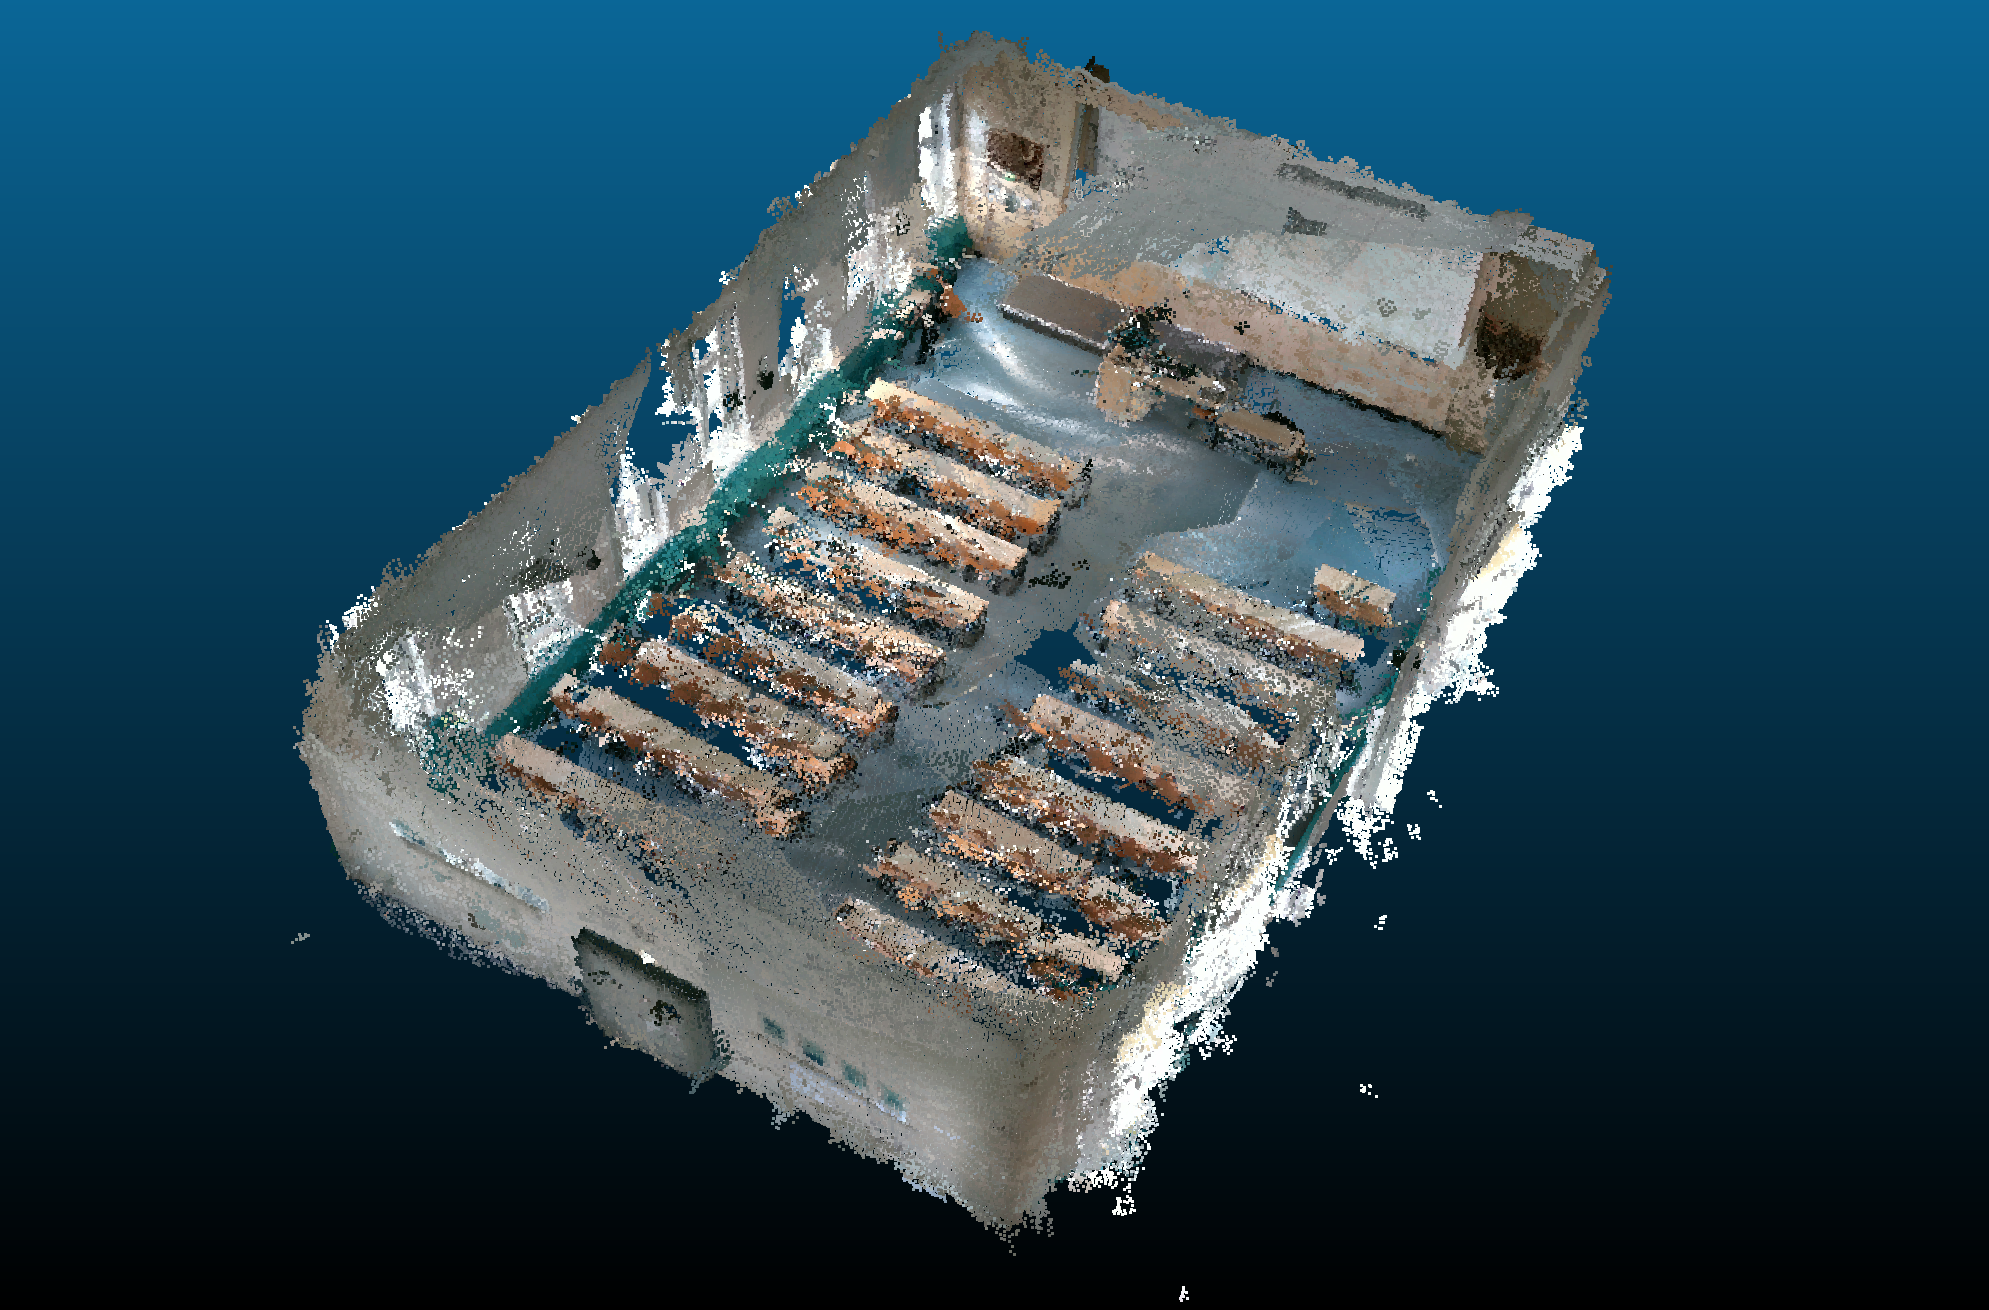
\includegraphics[width=.9\linewidth]{images/307.png}
        \caption[Dynamic Dataset - auditorium]{}
        \label{fig:fin307}
    \end{subfigure}
    \begin{subfigure}{0.5\textwidth}
        \centering
        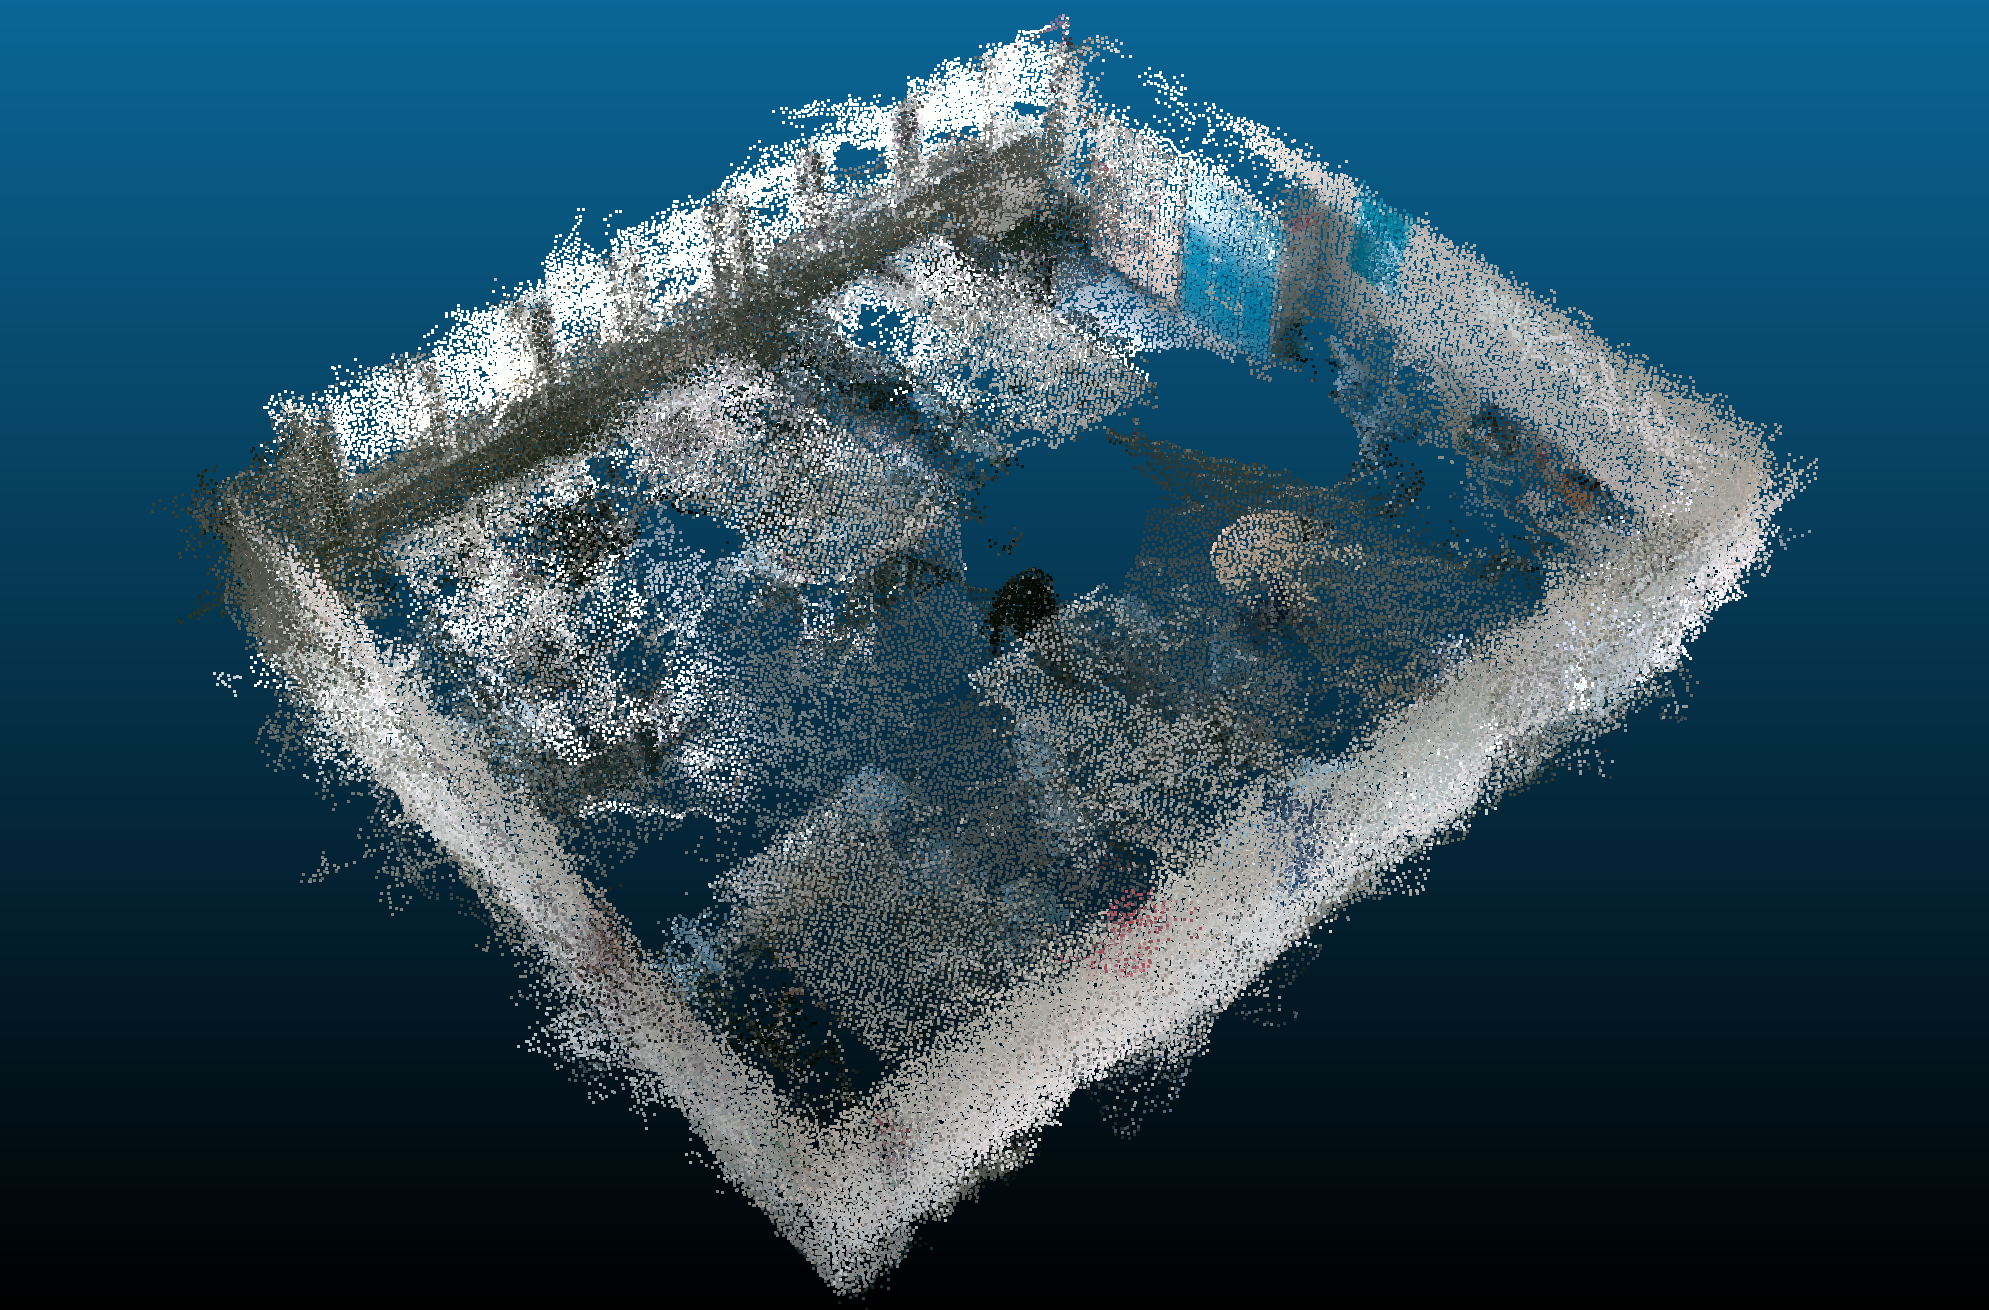
\includegraphics[width=.9\linewidth]{images/333.png}
        \caption[Dynamic Dataset - conference room]{}
        \label{fig:fin333}
    \end{subfigure}
    \begin{subfigure}{0.5\textwidth}
        \centering
        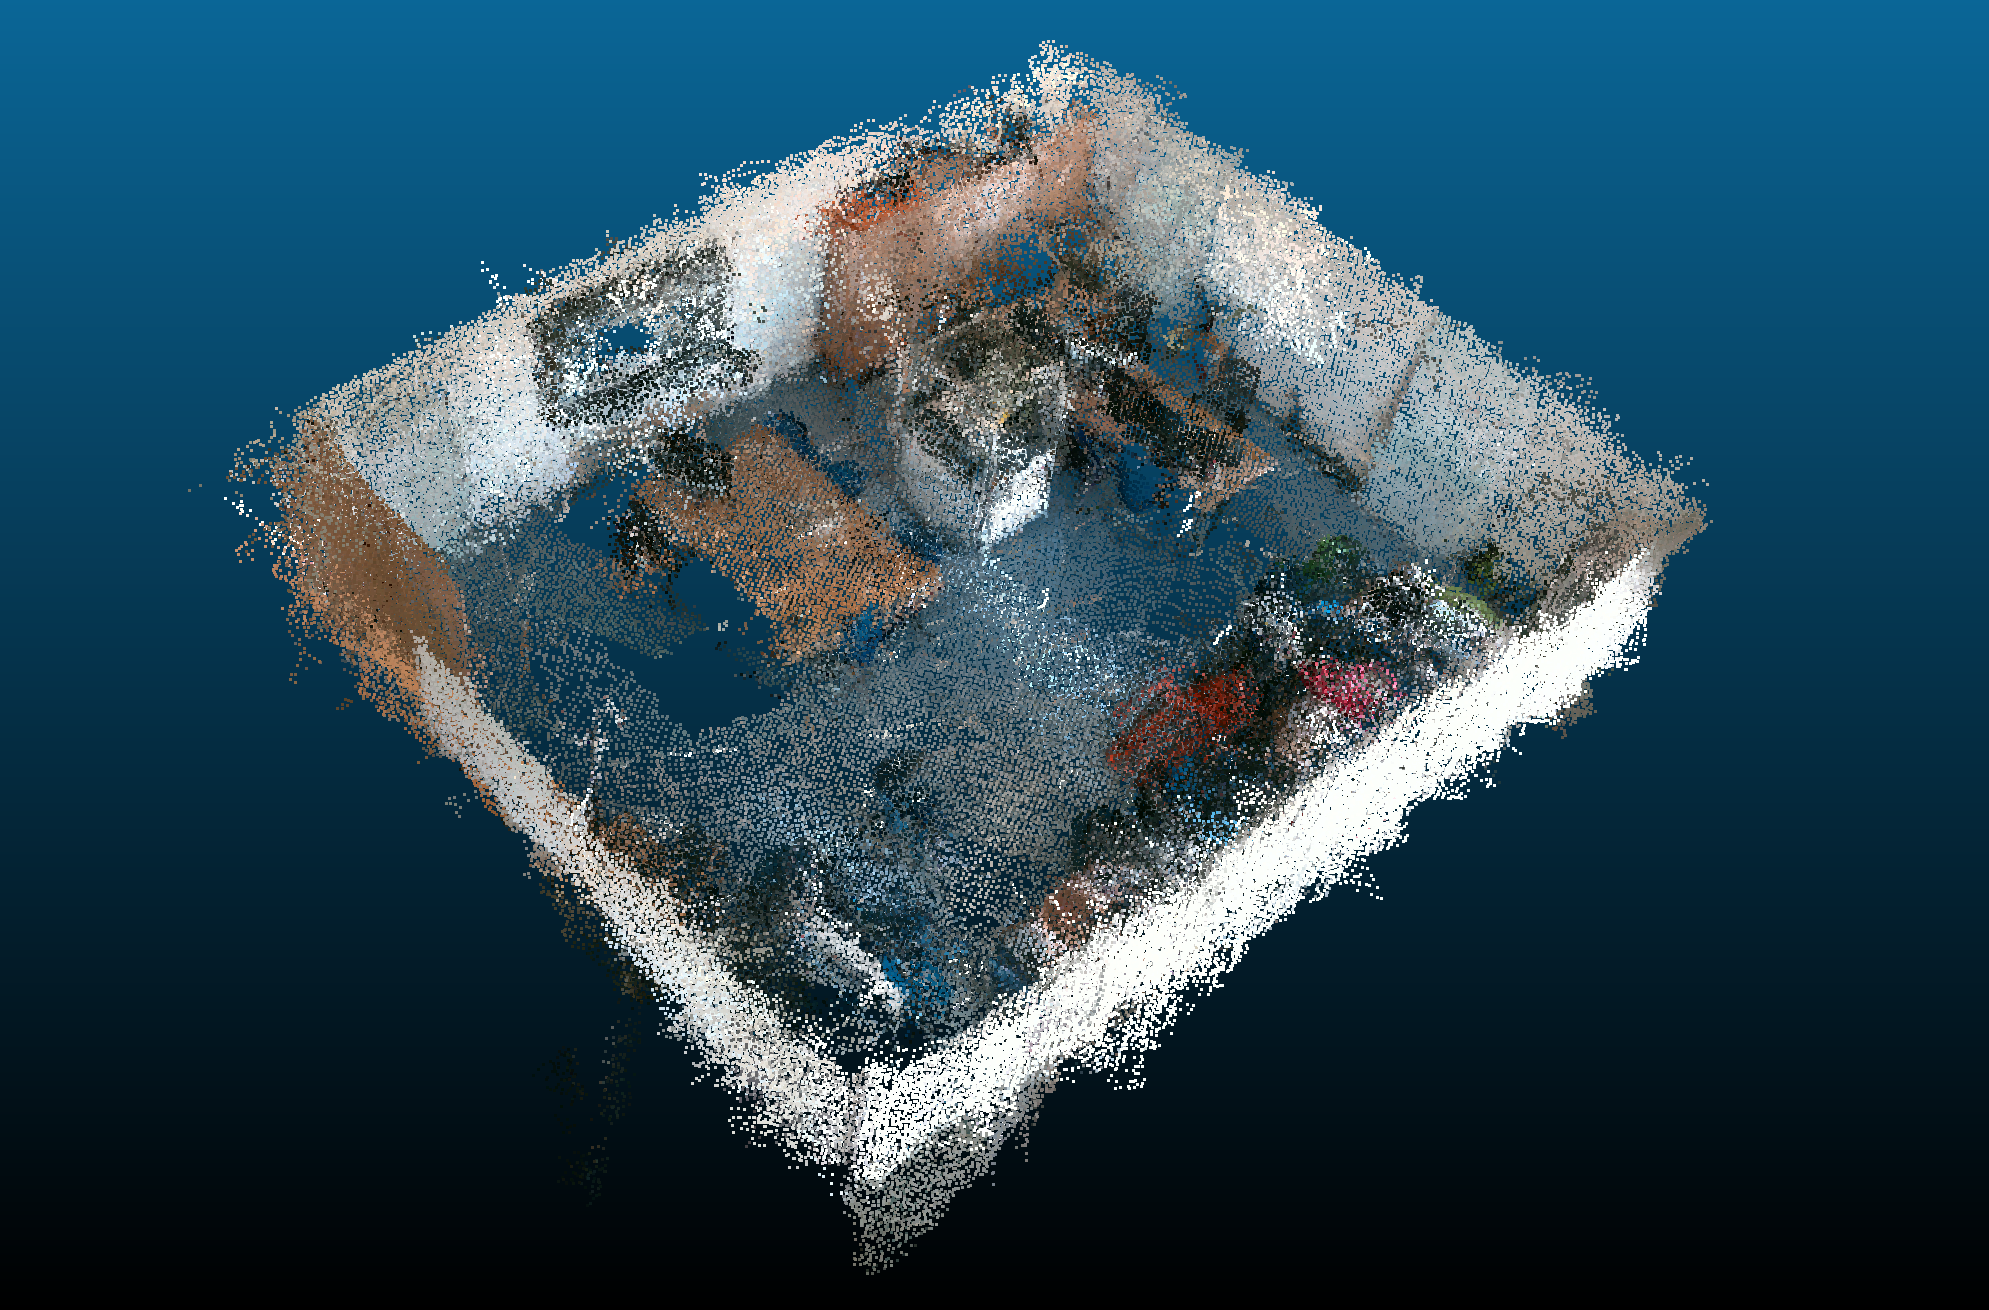
\includegraphics[width=0.9\linewidth]{images/425.png}
        \caption[Dynamic Dataset office]{}
        \label{fig:fin425}
    \end{subfigure}
    \begin{subfigure}{0.5\textwidth}
        \centering
        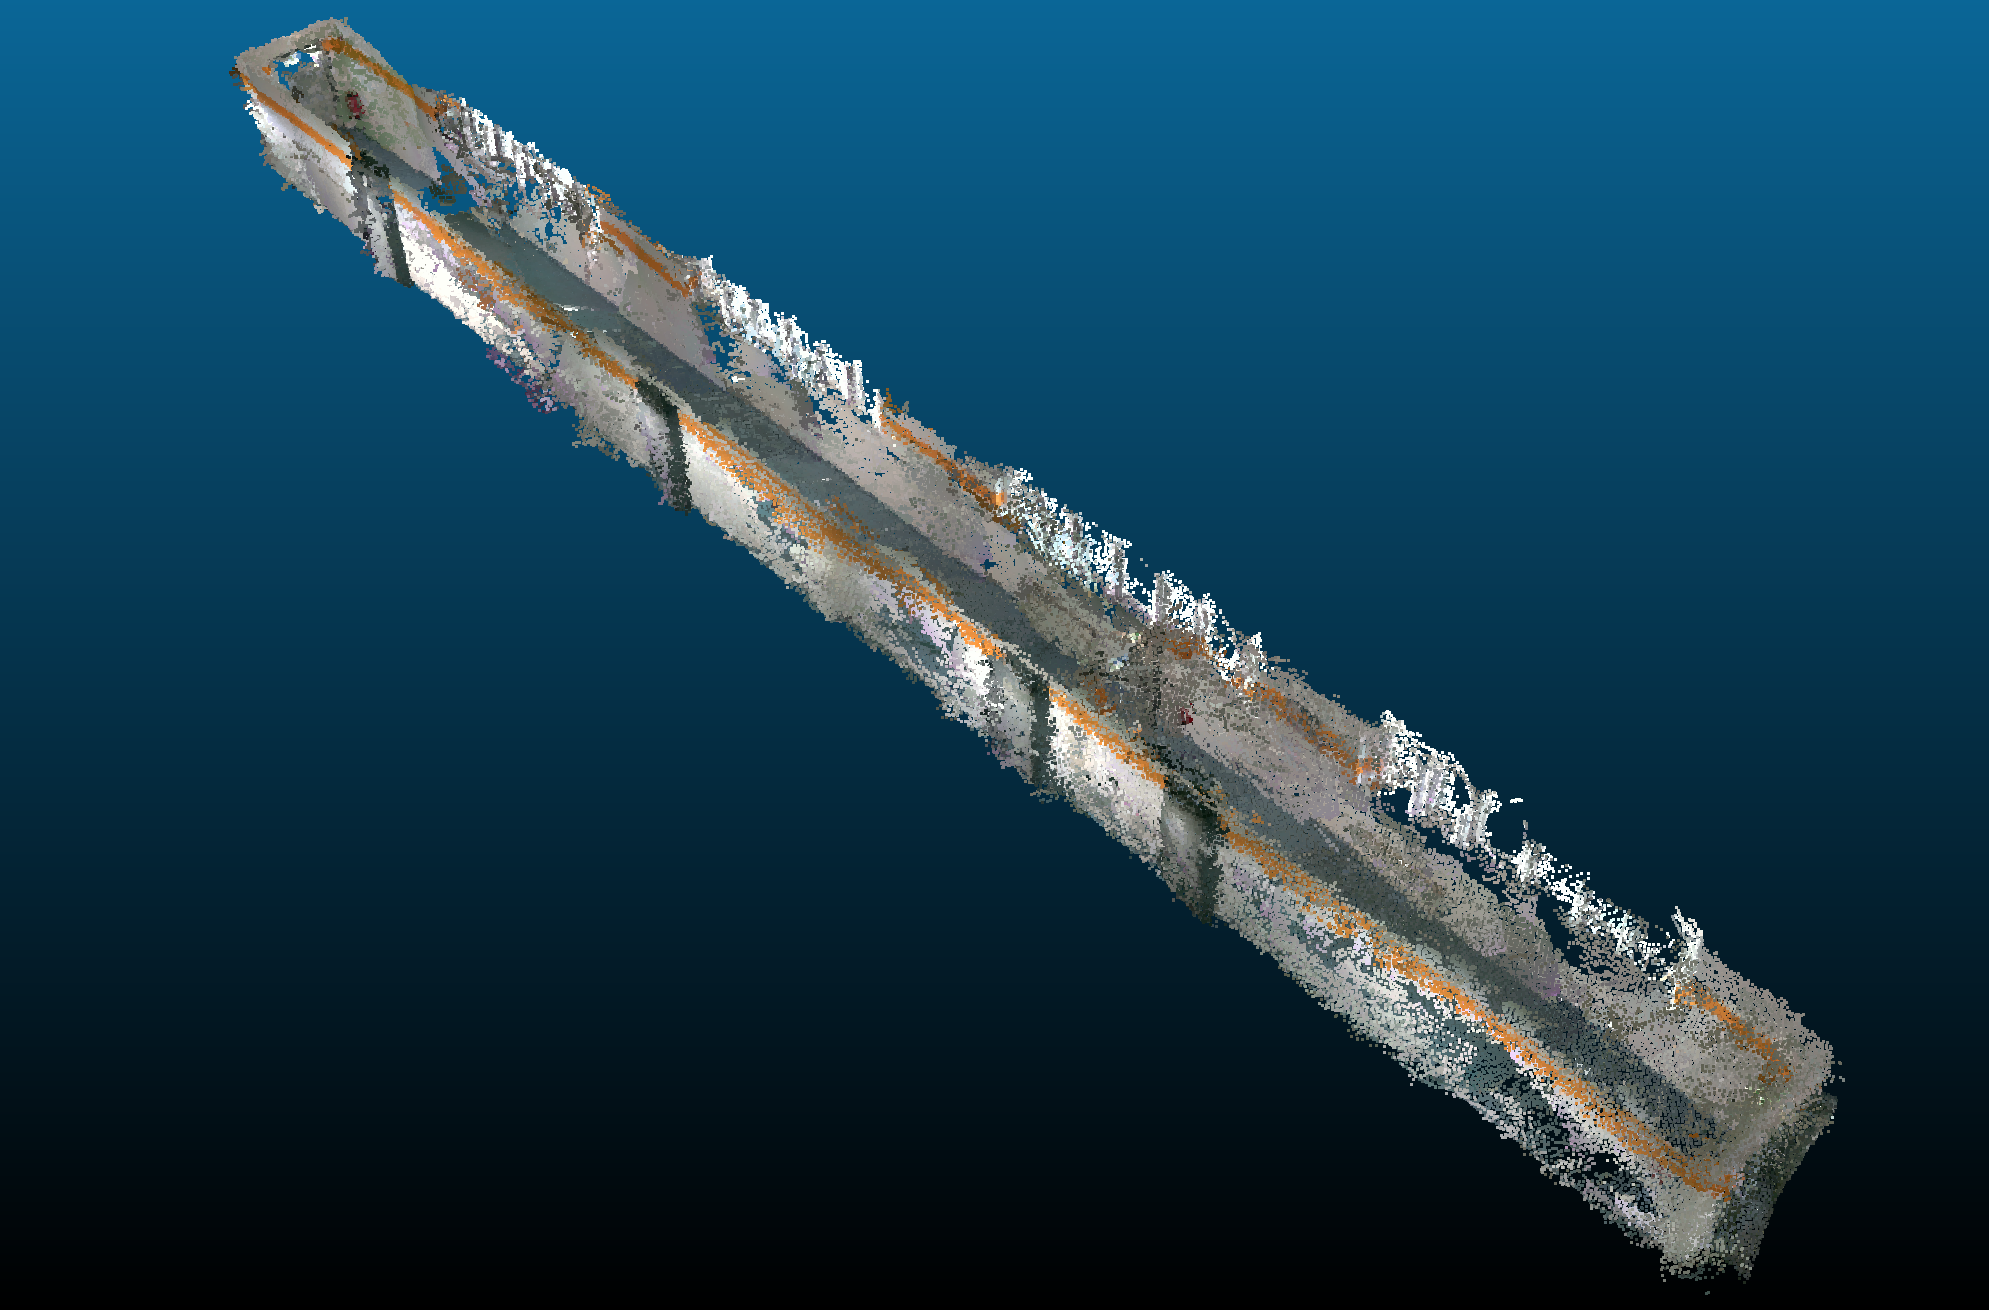
\includegraphics[width=0.9\linewidth]{images/hallway.png}
        \caption[Dynamic Dataset office]{}
        \label{fig:finhw}
    \end{subfigure}
    \caption[Dynamic Datasets]{The recordings for each scene type: (a)auditorium, (b) conference room, (c) office and (d) hallway.}
    \label{fig:fin}
\end{figure}

Since no ground truth exists for a novel dataset like this, we create a set of ground truth planes $gt_{end}$ for only the most recent update of each scene, e.g., for the entire recording.
To prepare for the evaluation of a map $m_t$ at a given time $t$, we crop all planes in $gt_{end}$ by removing all points that are not present in $m_t$, as shown in
Figure~\ref{fig:dynGT}.
We speed up this expensive process by employing a KD-Tree neighbor search with a small search radius since we only need to know whether a certain point is present or not.
% Furthermore, we remove planes from the ground truth if the number of included points falls short of a threshold. 
\begin{figure}[H]
    \centering
    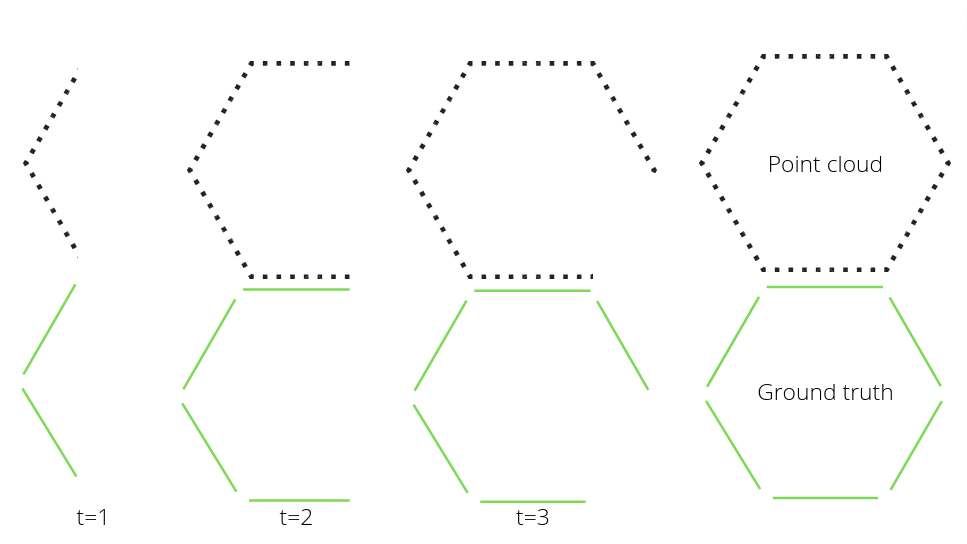
\includegraphics[width=15 cm]{images/dynamic_eval.png}
    \caption[Dynamic Ground Truth Generation]{Dynamic ground truth generation. All planes that are included in \textit{Ground Truth} are cropped depending on
        the available point cloud at each time \textit{t} }
    \label{fig:dynGT}
\end{figure}


\section{Definition Real-Time}\label{sec:realtime}
% FIXME "wirkt etwas komisch hier. bin mir noch unsicher." 
To determine whether or not an algorithm runs in real-time, we must first define the meaning of real-time.

We have to consider possible hardware limitations, data flow, and simply
how often it is needed to perform calculations in correspondence with the given use case.

%TODO Gar nicht mehr unbedingt nötig, wenn die obere grenze eh der SLAM ist, oder? 
%  The D455 has a depth frame rate of up to 90, while the T265 only achieves a maximum frame rate of 30
The recorded raw data is not directly sent to the plane detection algorithm but instead given to RTAB-MAP, which then performs
calculations to update and publish the map.
Therefore, the upper limit is the frequency of how often RTAB-MAP publishes those updates, which by default is once per second.
According to this upper limit, we consider an algorithm \textit{real-time applicable}, if it achieves an average frame
rate of minimum 1, e.g., the algorithm manages to process the entire point cloud and detect all planes within one second.

%TODO  Eig nur needed wenn die algos langsamer sind als 1s ODER sollte die cloud extrem wachsen kann man sich auf die 6 meter beschränken, erstmal aber nicht}\\
% \subsection*{reduktion (opt)}
% We can reduce complexity further by taking the specifications (background)
% of the D455 into account. The RMS error of the D455 is reported to be 2\% at 4 meters distance to the sensor.
% Furthermore, the ideal distance is stated to range between $0.6 - 6$ meters.
% To maintain a dense and precise representation of our environment, we therefore limit the detection of planes to a
% radius of 6 meters from the current position.

\section{Summary}
Many applications have constraints in the form of a temporal component. Applications that include plane detection
are no exception. In addition to time constraints, good quality is usually tightly coupled to expensive sensors.
To evaluate to what extent it is possible to perform precise plane detection with a real-time constraint on off-the shelf hardware,
we compare selected algorithms.

\end{document}